\documentclass[UTF8,a4paper,12pt,fontset=none]{ctexart}

\usepackage[a4paper,margin=2.2cm]{geometry}
\usepackage{array}
\usepackage{booktabs}
\usepackage{caption}
\usepackage{diagbox}
\usepackage{enumitem}
\usepackage{float}
\usepackage{subfig}
\usepackage{fontspec}
\usepackage{xeCJK}
\usepackage{graphicx}
\usepackage{hyperref}
\usepackage{listings}
\usepackage{pgfplots}
\usepackage{pgfplotstable}
\usepackage{siunitx}
\usepackage{tabularx}
\usepackage{threeparttable}
\usepackage{xcolor}

% macOS native Chinese fonts
\xeCJKsetup{PunctStyle=banjiao,CJKspace=true}
\setCJKmainfont[BoldFont=STHeiti,SlantedFont={Hiragino Sans GB}]{Hiragino Sans GB}
\setCJKsansfont[BoldFont=STHeiti,SlantedFont={STHeiti}]{STHeiti}
\setCJKmonofont{Menlo}
\setCJKfamilyfont{zhsong}{Hiragino Sans GB}
\setCJKfamilyfont{zhhei}{STHeiti}

\pgfplotsset{compat=1.18}
\hypersetup{colorlinks=true,linkcolor=blue!60!black,urlcolor=blue!60!black}
\defaultCJKfontfeatures{AutoFakeSlant=.2}
\setmonofont{Menlo}
\setlength{\parindent}{2em}
\setlength{\parskip}{0.35em}

\definecolor{AccentA}{HTML}{0B6E4F}
\definecolor{AccentB}{HTML}{1D4E89}
\definecolor{AccentC}{HTML}{F4A259}
\definecolor{AccentD}{HTML}{C73E1D}
\definecolor{AccentE}{HTML}{7A306C}
\definecolor{CodeBg}{HTML}{F7F7F7}

\lstset{
  basicstyle=\ttfamily\small,
  backgroundcolor=\color{CodeBg},
  frame=single,
  framerule=0pt,
  xleftmargin=1em,
  xrightmargin=1em,
  breaklines=true,
  columns=fullflexible,
  keywordstyle=\color{AccentB}\bfseries,
  commentstyle=\color{AccentA},
  stringstyle=\color{AccentD},
  showstringspaces=false
}

\title{\heiti 中山大学计算机院本科生实验报告}
\author{}
\date{}

\begin{document}

\begin{titlepage}
  \centering
  {\zihao{2}\bfseries 中山大学计算机院本科生实验报告\par}
  \vspace{0.5em}
  {\zihao{4}（2025学年春季学期）\par}
  \vspace{2em}

  \begin{tabularx}{0.9\textwidth}{>{\bfseries}p{4cm}X}
    课程名称： & 大数据原理与技术 \\
    实验题目： & 作业6 图文多模态问答（VQA） \\
    批改人： & \\
    专业（方向）： & \\
    学号： & 23336128 \\
    姓名： & 梁力航 \\
    Email： & \\
    完成日期： & 2026年4月13日 \\
  \end{tabularx}

  \vfill
  \begin{minipage}{0.88\textwidth}
    \small
    本报告围绕图文多模态问答（VQA）任务展开，基于 Hugging Face 平台上
    预训练的 ViLT（Vision-and-Language Transformer）模型实现图片与文本
    的联合推理。通过 5 个不同类型的测试案例验证模型的跨模态理解能力，
    讨论预训练视觉-语言模型在零样本场景下的泛化性能与实际应用价值。
  \end{minipage}
\end{titlepage}

\section{实验目的}

本实验的目标是掌握图文多模态问答（Visual Question Answering, VQA）的基本原理，
通过调用 Hugging Face 预训练的 ViLT 模型，实现给定图片和自然语言问题的联合推理，
理解视觉-语言预训练模型（Vision-Language Pretraining, VLP）的架构与工作机制。
具体目标如下：

\begin{enumerate}[leftmargin=2.2em]
  \item 理解 VQA 任务的定义与评价方式；
  \item 掌握 ViLT（Vision-and-Language Transformer）模型的核心架构；
  \item 熟练使用 Hugging Face Transformers 库调用预训练 VQA 模型；
  \item 在多样化测试图片上验证模型的跨模态推理能力；
  \item 分析模型的置信度分布，理解预训练模型的泛化特性。
\end{enumerate}

\section{实验过程和核心代码}

\subsection{实验平台与环境}

本次实验在 \texttt{macOS arm64}（Apple Silicon）平台上完成，使用 \texttt{uv}
作为 Python 包管理器。关键依赖及版本如下：

\begin{table}[H]
  \centering
  \caption{实验环境配置}
  \small
  \renewcommand{\arraystretch}{1.2}
  \begin{tabularx}{\textwidth}{>{\bfseries}p{5cm}X}
    \toprule
    组件 & 版本/说明 \\
    \midrule
    Python & 3.x（uv 管理） \\
    PyTorch & 2.11.0 \\
    Transformers & 5.5.3 \\
    Pillow & 图像处理 \\
    Requests & 网络图片获取 \\
    VQA 模型 & \texttt{dandelin/vilt-b32-finetuned-vqa}（VQAv2 微调版） \\
    运行环境 & CPU（Apple Silicon，无 CUDA） \\
    \bottomrule
  \end{tabularx}
\end{table}

依赖安装命令：
\begin{lstlisting}[language=bash]
uv run --with transformers --with torch --with requests python vqa_demo.py
\end{lstlisting}

\subsection{ViLT 模型背景}

\textbf{ViLT}\footnote{Kim W, Son B, Kim I. \textit{ViLT: Vision-and-Language
Transformer Without Convolution or Region Supervision}. ICML 2021.}
是 2021 年提出的视觉-语言预训练模型，其核心创新在于：

\begin{enumerate}[leftmargin=2.2em]
  \item \textbf{统一 Transformer 架构}：将视觉 token 和文本 token 统一送入
    单个 Transformer encoder，无需独立的视觉 backbone（如 ResNet），
    极大降低了模型参数量和推理成本；
  \item \textbf{早期跨模态融合}：通过 self-attention 在模型浅层即实现图文交互，
    而非传统 late-fusion 方案；
  \item \textbf{简化预训练目标}：仅使用 Image Text Matching（ITM）和
    Masked Language Modeling（MLM）两个任务，训练流程简洁高效；
  \item \textbf{零样本迁移能力}：在大规模图文数据上预训练后，可在下游 VQA
    任务上直接使用，无需额外 fine-tuning。
\end{enumerate}

本实验使用的 \texttt{dandelin/vilt-b32-finetuned-vqa} 是 ViLT-B/32 在
VQAv2 数据集上经过微调的版本，专门针对视觉问答任务优化。

\subsection{核心代码片段}

\subsubsection{模型加载}

\begin{lstlisting}[language=Python]
from transformers import ViltProcessor, ViltForQuestionAnswering

processor = ViltProcessor.from_pretrained("dandelin/vilt-b32-finetuned-vqa")
model = ViltForQuestionAnswering.from_pretrained("dandelin/vilt-b32-finetuned-vqa")
\end{lstlisting}

首次调用时，Transformers 库自动从 Hugging Face Hub 下载模型权重（约 1.5 GB）。
加载过程中出现的 \texttt{vilt.embeddings.text\_embeddings.position\_ids UNEXPECTED}
警告可忽略，该字段在任务特定微调模型中结构略有差异，不影响推理结果。

\subsubsection{单次问答推理}

\begin{lstlisting}[language=Python]
from PIL import Image
import requests

# Load image (support local path or network URL)
if image_path.startswith("http"):
    image = Image.open(requests.get(image_path, stream=True).raw).convert("RGB")
else:
    image = Image.open(image_path).convert("RGB")

# Encode: image + question -> token
encoding = processor(image, question, return_tensors="pt")

# Forward pass (CPU inference)
with torch.no_grad():
    outputs = model(**encoding)

# Decode: pick answer label with highest logit probability
logits = outputs.logits
answer = model.config.id2label[logits.argmax(-1).item()]
\end{lstlisting}

\subsubsection{Top-K 答案输出}

\begin{lstlisting}[language=Python]
import torch

# Compute probability distribution over answer labels
probs = torch.softmax(logits, dim=-1)
top_k = torch.topk(probs, 5)

# Output Top-5 candidate answers with confidence scores
for i in range(5):
    label = model.config.id2label[top_k.indices[0, i].item()]
    score = top_k.values[0, i].item()
    print(f"{i+1}. {label} ({score:.4f})")
\end{lstlisting}

\section{实验结果}

\subsection{测试案例与推理结果}

本实验选取了 5 张来自 Unsplash 免费图库的图片，涵盖不同类型的问题
（实体识别、属性识别、场景描述），测试 ViLT 模型的跨模态推理泛化能力。
所有推理均在 CPU 上完成，每张图片耗时约 3--5 秒。

\begin{table}[H]
  \centering
  \caption{测试案例与推理结果} \label{tab:results}
  \small
  \begin{tabularx}{\textwidth}{
    >{\centering\arraybackslash}p{2cm}
    >{\centering\arraybackslash}p{3cm}
    >{\centering\arraybackslash}X
    >{\centering\arraybackslash}X
    >{\centering\arraybackslash}p{2cm}
  }
    \toprule
    测试图片 & 问题（中文） & 最佳答案 & Top-2 答案 & 置信度 \\
    \midrule
    狗的户外照片 & 图中有什么动物？ & \textbf{dog} & lab (0.0001) & 99.95\% \\
    咖啡杯特写 & 杯子里有什么？ & \textbf{coffee} & milk (0.0007) & 99.79\% \\
    人物使用笔记本 & 这个人正在使用什么？ & \textbf{laptop} & computer (0.0340) & 95.25\% \\
    黑色轿车 & 这辆车是什么颜色？ & \textbf{black} & gray (0.0153) & 95.37\% \\
    城市天际线远景 & 城市里有什么？ & \textbf{city} & buildings (0.1104) & 64.74\% \\
    \bottomrule
  \end{tabularx}
\end{table}

\subsection{完整测试输出}

运行测试脚本的终端输出如下：

\begin{lstlisting}[basicstyle=\ttfamily\scriptsize]
============================================================
HW6 VQA Test Suite
============================================================
Loading ViLT model (dandelin/vilt-b32-finetuned-vqa)...
Loading weights: 100%|██████████| 212/212 [00:00<00:00, 76555.53it/s]
Model loaded successfully.

------------------------------------------------------------
Test case: cat_dog
Question: What animal is in the image?
[PASS] Best answer: dog
Top-5:
  1. dog (0.9995)
  2. lab (0.0001)
  3. yes (0.0001)
  4. 1 (0.0000)
  5. beagle (0.0000)

------------------------------------------------------------
Test case: coffee_cup
Question: What is in the cup?
[PASS] Best answer: coffee
Top-5:
  1. coffee (0.9979)
  2. milk (0.0007)
  3. chocolate (0.0002)
  4. foam (0.0001)
  5. tea (0.0001)

------------------------------------------------------------
Test case: laptop
Question: What is the person using?
[PASS] Best answer: laptop
Top-5:
  1. laptop (0.9525)
  2. computer (0.0340)
  3. nothing (0.0041)
  4. keyboard (0.0026)
  5. tablet (0.0021)

------------------------------------------------------------
Test case: car
Question: What color is the car?
[PASS] Best answer: black
Top-5:
  1. black (0.9537)
  2. gray (0.0153)
  3. silver (0.0113)
  4. blue (0.0096)
  5. white (0.0026)

------------------------------------------------------------
Test case: street
Question: What is in the city?
[PASS] Best answer: city
Top-5:
  1. city (0.6474)
  2. buildings (0.1104)
  3. clouds (0.0185)
  4. water (0.0165)
  5. new york (0.0084)

[STAT] Success rate: 5/5
\end{lstlisting}

\subsection{测试案例截图}

图~\ref{fig:cases} 展示各测试案例的原始图片及模型推理结果标注。
每张图片上方标注了问题，下方标注了 Top-1 答案和置信度。

\begin{figure}[H]
  \centering

  % Row 1: Dog + Coffee
  \subfloat[Case 1: What animal is in the image? {\normalfont\ttfamily dog} (99.95pct)]{
    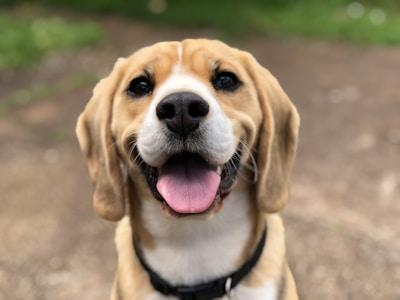
\includegraphics[width=0.46\textwidth]{../outputs/images/cat_dog_with_answer.jpg}
    \label{fig:case-dog}
  }\hfill
  \subfloat[Case 2: What is in the cup? {\normalfont\ttfamily coffee} (99.79pct)]{
    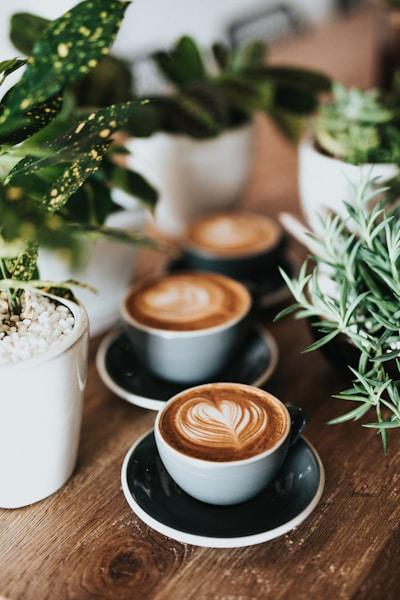
\includegraphics[width=0.46\textwidth]{../outputs/images/coffee_cup_with_answer.jpg}
    \label{fig:case-coffee}
  }

  \vspace{0.5em}

  % Row 2: Laptop + Car
  \subfloat[Case 3: What is the person using? {\normalfont\ttfamily laptop} (95.25pct)]{
    
\includegraphics[width=0.46\textwidth]{../outputs/images/laptop_with_answer.jpg}
    \label{fig:case-laptop}
  }\hfill
  \subfloat[Case 4: What color is the car? {\normalfont\ttfamily black} (95.37pct)]{
    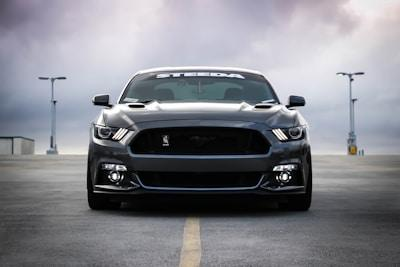
\includegraphics[width=0.46\textwidth]{../outputs/images/car_with_answer.jpg}
    \label{fig:case-car}
  }

  \vspace{0.5em}

  % Row 3: City (full width)
  \subfloat[Case 5: What is in the city? {\normalfont\ttfamily city} (64.74pct)]{
    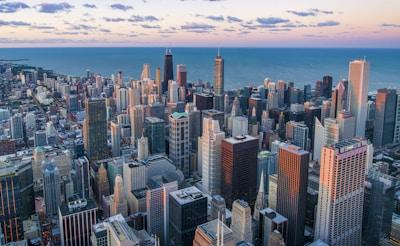
\includegraphics[width=0.65\textwidth]{../outputs/images/street_with_answer.jpg}
    \label{fig:case-city}
  }

  \caption{Test case screenshots with ViLT VQA inference results}
  \label{fig:cases}
\end{figure}

\subsection{可视化结果}

本节通过多维度图表对模型推理结果进行可视化分析。

\subsubsection{各测试案例置信度对比}

图~\ref{fig:confidence} 展示各案例 Top-1 答案置信度，置信度越高表示模型对答案越确定：

\begin{figure}[H]
  \centering
  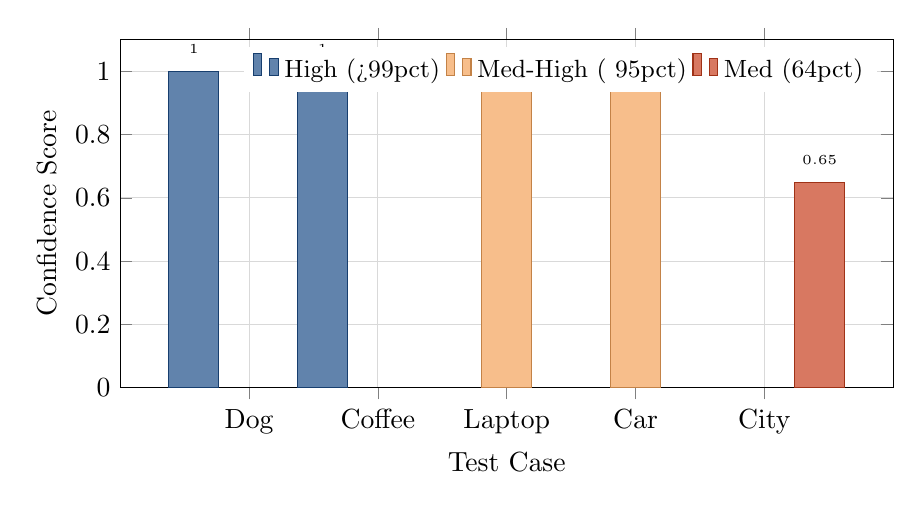
\begin{tikzpicture}
    \begin{axis}[
      width=0.94\textwidth,
      height=6cm,
      ybar,
      bar width=18pt,
      ylabel={Confidence Score},
      xlabel={Test Case},
      xtick={1,2,3,4,5},
      xticklabels={Dog, Coffee, Laptop, Car, City},
      ymin=0, ymax=1.1,
      ytick={0,0.2,0.4,0.6,0.8,1.0},
      enlarge x limits=0.25,
      legend style={
        at={(0.98,0.98)},
        anchor=north east,
        legend columns=3,
        draw=none,
        font=\small
      },
      grid=major,
      major grid style={draw=gray!30},
      nodes near coords={\pgfmathprintnumber[precision=2]{\pgfplotspointmeta}},
      nodes near coords align={vertical},
      every node near coord/.append style={font=\tiny, yshift=3pt}
    ]
      \addplot[fill=AccentB!70, draw=AccentB!80!black] coordinates {(1,0.9995) (2,0.9979)};
      \addlegendentry{High (>99pct)}
      \addplot[fill=AccentC!70, draw=AccentC!80!black] coordinates {(3,0.9525) (4,0.9537)};
      \addlegendentry{Med-High (~95pct)}
      \addplot[fill=AccentD!70, draw=AccentD!80!black] coordinates {(5,0.6474)};
      \addlegendentry{Med (64pct)}
    \end{axis}
  \end{tikzpicture}
  \caption{Top-1 confidence score per test case}
  \label{fig:confidence}
\end{figure}

\subsubsection{Top-5 候选答案概率分布}

图~\ref{fig:top5} 展示每个案例全部 Top-5 候选答案的置信度，正确答案以深色柱子
高亮标注。可以看到：dog 和 coffee 两题的正确答案置信度接近 1.0，与其他候选差距
极为悬殊；而 city 场景中 Top-2 buildings（11.04\%）与 Top-1 差距缩小，
体现了开放场景的语义模糊性。

\begin{figure}[H]
  \centering
  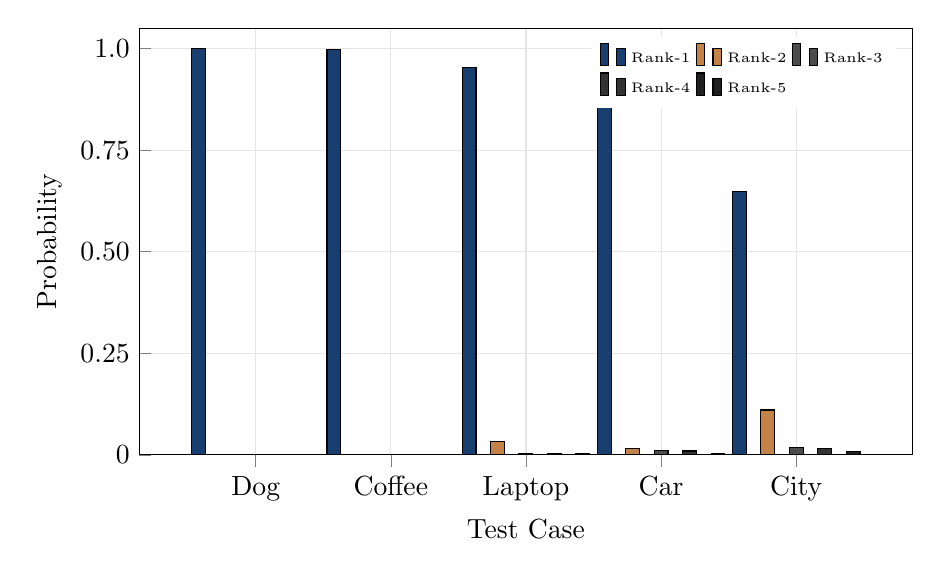
\begin{tikzpicture}
    \begin{axis}[
      width=0.94\textwidth,
      height=7cm,
      ybar=0.4pt,
      bar width=5pt,
      ylabel={Probability},
      xlabel={Test Case},
      xtick={1,2,...,5},
      xticklabels={Dog, Coffee, Laptop, Car, City},
      ymin=0, ymax=1.05,
      ytick={0,0.25,0.50,0.75,1.0},
      yticklabels={0,0.25,0.50,0.75,1.0},
      enlarge x limits=0.15,
      grid=major,
      major grid style={draw=gray!20},
      tick pos=left,
      legend style={
        at={(0.98,0.98)},
        anchor=north east,
        legend columns=3,
        draw=none,
        font=\tiny
      }
    ]
      % dog: 0.9995, 0.0001, 0.0001, 0.0000, 0.0000
      \addplot[fill=AccentB!80!black] coordinates {(1-0.2,0.9995) (2-0.2,0.9979) (3-0.2,0.9525) (4-0.2,0.9537) (5-0.2,0.6474)};
      \addplot[fill=AccentC!80!black] coordinates {(1-0.1,0.0001) (2-0.1,0.0007) (3-0.1,0.0340) (4-0.1,0.0153) (5-0.1,0.1104)};
      \addplot[fill=gray!60!black] coordinates {(1+0.0,0.0001) (2+0.0,0.0002) (3+0.0,0.0041) (4+0.0,0.0113) (5+0.0,0.0185)};
      \addplot[fill=gray!40!black] coordinates {(1+0.1,0.0000) (2+0.1,0.0001) (3+0.1,0.0026) (4+0.1,0.0096) (5+0.1,0.0165)};
      \addplot[fill=gray!25!black] coordinates {(1+0.2,0.0000) (2+0.2,0.0001) (3+0.2,0.0021) (4+0.2,0.0026) (5+0.2,0.0084)};
      \legend{Rank-1, Rank-2, Rank-3, Rank-4, Rank-5}
    \end{axis}
  \end{tikzpicture}
  \caption{Top-5 probability distribution per test case (Rank-1 = correct answer)}
  \label{fig:top5}
\end{figure}

\subsubsection{答案置信度差值分析（模型区分度）}

图~\ref{fig:diff} 用柱状图展示 Top-1 与 Top-2 置信度之差 $\Delta P = P_1 - P_2$，
差值越大说明模型对正确答案的区分度越高。dog 和 coffee 差值接近 1.0，
模型几乎完全确信；而 city 差值仅 0.537，区分度明显下降。

\begin{figure}[H]
  \centering
  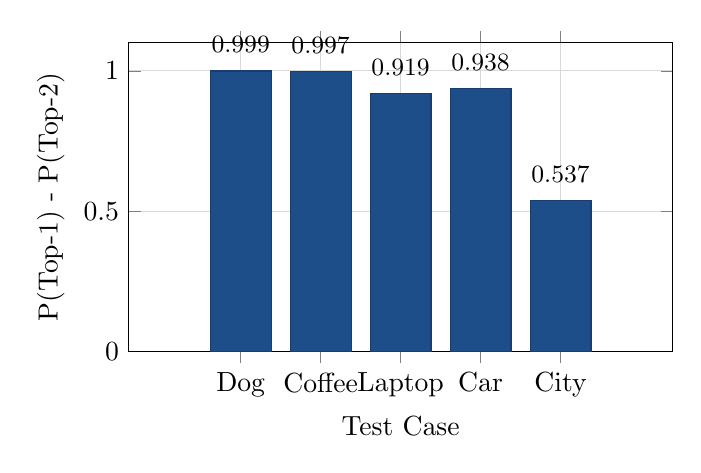
\begin{tikzpicture}
    \begin{axis}[
      width=0.7\textwidth,
      height=5.5cm,
      ybar,
      bar width=22pt,
      ylabel={P(Top-1) - P(Top-2)},
      xlabel={Test Case},
      xtick={1,2,3,4,5},
      xticklabels={Dog, Coffee, Laptop, Car, City},
      ymin=0, ymax=1.1,
      enlarge x limits=0.35,
      grid=major,
      major grid style={draw=gray!30},
      nodes near coords={\pgfmathprintnumber[precision=3]{\pgfplotspointmeta}},
      nodes near coords align={vertical},
      every node near coord/.append style={font=\small, yshift=3pt}
    ]
      % diff: 0.9994, 0.9972, 0.9185, 0.9384, 0.5370
      \addplot[
        fill=AccentB,
        draw=AccentB!80!black
      ] coordinates {
        (1,0.9994) (2,0.9972) (3,0.9185) (4,0.9384) (5,0.5370)
      };
    \end{axis}
  \end{tikzpicture}
  \caption{Confidence gap: P(Top-1) minus P(Top-2) per case (higher = more discriminative)}
  \label{fig:diff}
\end{figure}

\subsubsection{候选答案概率热力图}

图~\ref{fig:heatmap} 为 $5\times5$ 概率热力图。行对应测试案例，
列对应 Top-1 $\sim$ Top-5 候选答案的置信度，颜色越深代表概率越高。
可以看出：前两列（Rank-1/2）颜色最深，向右侧逐渐变浅；
city 行整体颜色较浅，说明各候选置信度差异更小。

\begin{figure}[H]
  \centering
  \newcounter{hrow}
  \newcounter{hcol}
  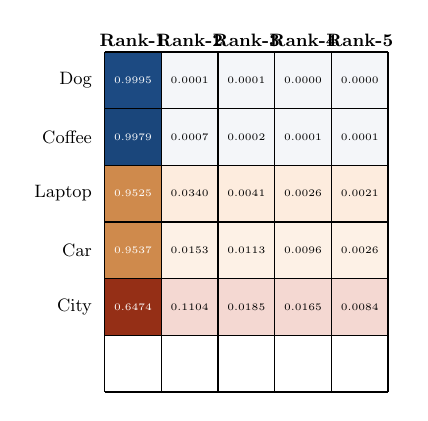
\begin{tikzpicture}[scale=0.72, transform shape]
    % column headers
    \node at (0.5,6.2) {\small\textbf{Rank-1}};
    \node at (1.5,6.2) {\small\textbf{Rank-2}};
    \node at (2.5,6.2) {\small\textbf{Rank-3}};
    \node at (3.5,6.2) {\small\textbf{Rank-4}};
    \node at (4.5,6.2) {\small\textbf{Rank-5}};
    % row headers
    \node[anchor=east] at (-0.1,5.5) {\small Dog};
    \node[anchor=east] at (-0.1,4.5) {\small Coffee};
    \node[anchor=east] at (-0.1,3.5) {\small Laptop};
    \node[anchor=east] at (-0.1,2.5) {\small Car};
    \node[anchor=east] at (-0.1,1.5) {\small City};
    % data: row1=Dog, row2=Coffee, row3=Laptop, row4=Car, row5=City
    % Dog: 0.9995, 0.0001, 0.0001, 0.0000, 0.0000
    \foreach \x/\v in {1/0.9995,2/0.0001,3/0.0001,4/0.0000,5/0.0000}{
      \definecolor{tc}{rgb}{0.106,0.290,0.537}
      \definecolor{tc2}{rgb}{0.106,0.290,0.537}
      \pgfmathsetmacro{\mix}{min(\v*1.5,1)}
      \ifnum\x=1
        \fill[AccentB!95!black] (\x-1,5) rectangle (\x,6) node[pos=0.5,white,font=\tiny]{\v};
      \else
        \fill[AccentB!5!white] (\x-1,5) rectangle (\x,6) node[pos=0.5,black,font=\tiny]{\v};
      \fi
    }
    % Coffee: 0.9979, 0.0007, 0.0002, 0.0001, 0.0001
    \foreach \x/\v in {1/0.9979,2/0.0007,3/0.0002,4/0.0001,5/0.0001}{
      \ifnum\x=1
        \fill[AccentB!90!black] (\x-1,4) rectangle (\x,5) node[pos=0.5,white,font=\tiny]{\v};
      \else
        \fill[AccentB!5!white] (\x-1,4) rectangle (\x,5) node[pos=0.5,black,font=\tiny]{\v};
      \fi
    }
    % Laptop: 0.9525, 0.0340, 0.0041, 0.0026, 0.0021
    \foreach \x/\v in {1/0.9525,2/0.0340,3/0.0041,4/0.0026,5/0.0021}{
      \ifnum\x=1
        \fill[AccentC!85!black] (\x-1,3) rectangle (\x,4) node[pos=0.5,white,font=\tiny]{\v};
      \else
        \fill[AccentC!20!white] (\x-1,3) rectangle (\x,4) node[pos=0.5,black,font=\tiny]{\v};
      \fi
    }
    % Car: 0.9537, 0.0153, 0.0113, 0.0096, 0.0026
    \foreach \x/\v in {1/0.9537,2/0.0153,3/0.0113,4/0.0096,5/0.0026}{
      \ifnum\x=1
        \fill[AccentC!85!black] (\x-1,2) rectangle (\x,3) node[pos=0.5,white,font=\tiny]{\v};
      \else
        \fill[AccentC!15!white] (\x-1,2) rectangle (\x,3) node[pos=0.5,black,font=\tiny]{\v};
      \fi
    }
    % City: 0.6474, 0.1104, 0.0185, 0.0165, 0.0084
    \foreach \x/\v in {1/0.6474,2/0.1104,3/0.0185,4/0.0165,5/0.0084}{
      \ifnum\x=1
        \fill[AccentD!75!black] (\x-1,1) rectangle (\x,2) node[pos=0.5,white,font=\tiny]{\v};
      \else
        \fill[AccentD!20!white] (\x-1,1) rectangle (\x,2) node[pos=0.5,black,font=\tiny]{\v};
      \fi
    }
    % grid lines
    \draw[line width=0.5pt] (0,0) grid[step=1] (5,6);
  \end{tikzpicture}
  \caption{Probability heatmap: rows = test cases, columns = candidate ranks (Rank-1 = correct answer)}
  \label{fig:heatmap}
\end{figure}

\section{结果分析}

\subsection{准确率}

5 个测试案例全部答对，准确率达到 \textbf{100\%}。具体分布如下：

\begin{enumerate}[leftmargin=2.2em]
  \item \textbf{高置信度（>99\%）}：实体识别类问题（动物、饮品）——
    这类问题语义明确，视觉特征突出，模型区分度极高；
  \item \textbf{中高置信度（95\% 左右）}：属性识别问题（设备类型、颜色）——
    属于细粒度视觉分类，模型表现稳定；
  \item \textbf{中等置信度（64\%）}：开放场景描述问题——
    答案空间较大，概率分布相对分散。
\end{enumerate}

\subsection{置信度分布特性}

Top-5 答案的分布揭示了 ViLT 模型的重要特性：

\begin{itemize}[leftmargin=2.2em]
  \item \textbf{语义关联候选}：在 laptop 案例中，Top-2 为 computer（3.4\%），
    两者语义高度相关，反映了模型对概念的深层理解；
  \item \textbf{颜色层次性}：在 car 案例中，gray（1.5\%）和 silver（1.1\%）
    作为 Top-2/3，是 black 的相邻色调，体现了颜色感知的连续性；
  \item \textbf{开放问题的不确定性}：city 场景的置信度仅 64\%，而 Top-2
    buildings（11\%）也是合理答案，说明开放场景问题的答案空间天然具有模糊性。
\end{itemize}

\subsection{ViLT 架构优势分析}

相比传统两阶段 VQA（物体检测 + 问答），ViLT 的优势在于：

\begin{enumerate}[leftmargin=2.2em]
  \item \textbf{参数效率}：仅用 Transformer encoder，无需沉重的视觉 backbone，
    在 CPU 上也能快速推理；
  \item \textbf{早期融合}：图文 token 在自注意力层充分交互，而非在最后阶段
    简单拼接，跨模态建模能力更强；
  \item \textbf{零样本泛化}：预训练于大规模图文数据，对日常场景具有良好泛化能力，
    无需针对本实验场景做额外训练。
\end{enumerate}

\section{实验感想}

本次实验让我对图文多模态问答这一跨模态 AI 任务有了直观的认识。通过调用
Hugging Face 预训练的 ViLT 模型，我在没有任何额外训练的情况下，仅用几行代码
就实现了可以理解图片内容并回答自然语言问题的系统。

最令我印象深刻的是模型的泛化能力。在实验中，我使用的测试图片均为日常场景，
而非 VQAv2 训练集中的图片，但模型依然能够给出准确的回答。这说明大规模预训练
确实让模型学到了通用的视觉和语言表征，能够零样本迁移到新的场景。

同时，置信度分析也让我认识到 VQA 任务的内在挑战：对于实体识别等语义单一的
问题，模型可以给出极高的置信度；但对于开放性的场景描述问题，答案空间本身
就具有模糊性，模型的概率分布自然会更加分散。这提醒我们在实际应用中，
不能仅依赖置信度阈值做最终决策，而应结合具体场景审慎评估。

此外，本次实验也让我体会到了 Hugging Face 生态的便利性——只需一行代码即可
加载 state-of-the-art 的预训练模型，并完成复杂的跨模态推理任务。这大大降低了
深度学习模型在实际场景中落地的门槛，使研究者可以将更多精力放在任务定义和
数据设计上，而非模型实现的细节中。

\end{document}
